\documentclass[12pt, a4paper, oneside]{report}

%% COMMANDS FOR THE TITLE PAGE CONTENT

% SW Author name (capitalized in its regular way)
\newcommand{\authorname}{Sean Allen Siegfreid R. Bugarin}

% SW Report Title (cannot exceed three lines)
% WORKING TITLE. The author chooses the final title.
\newcommand{\thetitle}{GroundLoop: A Self-Checking Agentic RAG System with Evaluation-Guided Recovery}

% Date of submission with normal capitalization.
% Use the format January 29, 2027.
% Fall 2026 final submission deadline per the Office of Signature Work guideline.
\newcommand{\submissiondate}{November 2, 2026}

% Mentor: First Name Last Name (normal capitalization)
\newcommand{\mentor}{Bing Luo}
% Mentor's Academic Unit (no abbreviations)
\newcommand{\mentoracademicunit}{Division of Natural and Applied Sciences}

% No co-mentor.
\newcommand{\comentor}{}

% Co-mentor's Academic Unit (no abbreviations)
% If the co-mentor is empty, the following will be ignored.
\newcommand{\comentoracademicunit}{}


%% PACKAGES

\usepackage[a4paper, margin=1in]{geometry}
\usepackage{parskip}

\usepackage{amsmath, amsthm}

% Office of Signature Work formatting: Times New Roman (or Garamond, Cambria,
% Arial) at 12 pt, double spaced, 1 inch margins. newtx supplies Times for
% text and math; amssymb is omitted because newtxmath provides its symbols.
\usepackage[T1]{fontenc}
\usepackage{newtxtext, newtxmath}
\renewcommand{\sfdefault}{\rmdefault}
\usepackage{graphicx}
\usepackage{float}
\usepackage{xcolor}
\usepackage{longtable, booktabs, array}

\usepackage{upquote}
\usepackage{microtype}

\usepackage{titlesec}
\titleformat{\chapter}[display]
  {\sffamily\bfseries\huge}
  {\Large\chaptertitlename\ \thechapter}
  {2ex}
  {\titlerule\vspace{1ex}\filright\MakeUppercase}
  [\vspace{1ex}\titlerule]
\titleformat{\section}{\normalfont\sffamily\Large\bfseries}{\thesection}{1em}{}
\titleformat{\subsection}{\normalfont\sffamily\large\bfseries}{\thesubsection}{1em}{}
\titleformat{\subsubsection}{\normalfont\sffamily\normalsize\bfseries}{\thesubsubsection}{1em}{}
% Tighter list and section spacing (layout only; text unchanged).
\usepackage{enumitem}
\setlist[itemize]{itemsep=0pt, topsep=2pt, parsep=0pt}
\titlespacing*{\section}{0pt}{2.5ex plus 1ex minus .2ex}{1.2ex plus .2ex}

\usepackage[style=numeric, sorting=none, url=false]{biblatex}
\addbibresource{references.bib}
% IEEE-like: numbered in order of first citation, each number bracketed
% separately ([8], [9], [10]), and hyphens in page ranges.
\DeclareCiteCommand{\cite}
  {\usebibmacro{prenote}}
  {\usebibmacro{citeindex}\mkbibbrackets{\usebibmacro{cite}}}
  {\multicitedelim}
  {\usebibmacro{postnote}}
\DefineBibliographyExtras{english}{\renewcommand*{\bibrangedash}{-}}

% Orange text inside the \instructions command must not appear
% in the final version of your report. You can either delete it
% from your document, or redefine the command \instructions, by
% commenting out the definition here...
\newcommand{\instructions}[1]{}
\newcommand{\authornote}[1]{}

\newcommand{\code}[1]{\texttt{\detokenize{#1}}}

\usepackage{tikz}
\usetikzlibrary{arrows.meta, positioning}

\usepackage[allcolors=blue, colorlinks=true]{hyperref}
\usepackage{xurl}
\usepackage{bookmark}

\urlstyle{same}

\usepackage{calc}
\usepackage{xifthen}
\usepackage{etoolbox}

\usepackage{setspace}

\begin{document}

\thispagestyle{empty}

% About Majors at DKU
Background:  Duke Kunshan University (DKU) is an interdisciplinary institution that grants dual undergraduate degrees, an MOE Chinese degree and a degree from Duke University in Durham, United States. The principal structure of DKU majors is robustly interdisciplinary. No student confines their study to a single discipline (for example, biology or economics). Instead, all students engage in broad inquiry related to a subject or question (for example, political economy or global health) and take a wide variety of courses related to that area (for example, in public policy, history, ethics, or economics). As a result, our graduates are prepared to engage in a wide variety of inquiries using multiple methodologies to address complex issues that require interdisciplinary approaches.  

This has implications for our vision and expectations of undergraduate theses and design projects, which reflect this broad interdisciplinary training. At DKU, every student completes a two-year project known as signature work which consists of multiple interconnected parts including thematic courses, experiential learning, capstones, and a final product. It seeks to integrate students’ interdisciplinary educational experience and culminates in the creation of a product in a scholarly, creative, or applied nature in lieu of an undergraduate thesis or design required by JED. Because DKU encourages students to cultivate their independence and creativity as one of its institutional student learning outcomes, the student-led signature work projects often reflect students’ own particular interdisciplinary interests and training.  In addition, signature work has an intensive emphasis on problem-solving and skill-development which is much needed for any interdisciplinary inquiry; thus, students’ final products are evidence of transferrable skills that students have acquired and demonstrated through the 2-year program, rather than content knowledge narrowly defined by disciplinary training. 
 
In sum, while the Chinese major declared with any given student might be construed narrowly, the experience of our students is much broader—and intentionally so.  This is a distinctive feature of our curriculum, and this distinctiveness results in broadly interdisciplinary submissions from our graduates’ submitting theses or design projects. We have designed this to prepare our students for a wide variety of graduate programs in China and the West, where interdisciplinary training is a competitive advantage.

%%%%%%%%%%%%%%%%%%%%%%%%%%%%%%%%%%%%%%%%%%%%%%%%%%%%%%%%%%%%%%%%

%% DO NOT CHANGE DIRECTLY THE CONTENTS OF THE TITLE PAGE.
%% TO CUSTOMIZE THE TITLE PAGE CHANGE THE DEFINITIONS OF THE COMMANDS
%% \authorname, \thetitle, \submissiondate
%% \mentor, \mentoracademicunit
%% \comentor, \comentoracademicunit

\begin{titlepage}

\vspace*{\bigskipamount}

\begin{center}
{\sffamily\LARGE\bfseries\MakeUppercase\thetitle\par}

\bigskip

by

\bigskip

{\Large \authorname}

\bigskip

Signature Work Product, in partial fulfillment of the \\
Duke Kunshan University Undergraduate Degree Program

\bigskip

\emph{\submissiondate}

\bigskip

Signature Work Program \\
Duke Kunshan University

\end{center}

\vfill

\textbf{\textsf{APPROVALS}}

\vspace{3em}\hrule\par
Mentor: \mentor, \mentoracademicunit

\ifthenelse{\equal{\comentor}{}}{}{
\vspace{3em}\hrule\par
Co-Mentor: \comentor, \comentoracademicunit
}

\end{titlepage}

%%%%%%%%%%%%%%%%%%%%%%%%%%%%%%%%%%%%%%%%%%%%%%%%%%%%%%%%%%%%%%%%

% Front matter
\clearpage
\pagenumbering{roman}

%%%%%%%%%%%%%%%%%%%%%%%%%%%%%%%%%%%%%%%%%%%%%%%%%%%%%%%%%%%%%%%%

% Only top-level units (chapters) should appear in the TOC
\setcounter{tocdepth}{0} 
\tableofcontents

\doublespacing % τοῖς κείνων ρήμασι πειθόμενοι

%%%%%%%%%%%%%%%%%%%%%%%%%%%%%%%%%%%%%%%%%%%%%%%%%%%%%%%%%%%%%%%%

\chapter*{Abstract}
\addcontentsline{toc}{chapter}{Abstract}

% Abstract in English

GroundLoop is a functional implementation of a question answering system
that operates on its own documents and checks its own answers. It takes
questions, retrieves passages and answers, scores the answer with a
language model judge and deterministic tests, diagnoses why it failed,
recovers by rewriting the question, widening retrieval, regenerating the
answer, or abstaining, verifies the result, and reports everything through
a web console. Every run is saved as a trace. The paper then explores how much
trust we can place in this self-check. GroundLoop was compared to a
retrieve-once baseline with 1, 2, and 4 passages and a plain 8 passage
baseline on three small collections (88 questions in total), three times. It
improved correct answers from 0.81 to 0.97 on one collection and to 1.00 on
the other two, with just one actual regression in 27 runs of the loop. The
8-passage baseline matched it for less than half the cost. The diagnosis
matched a gold class offline most of the time, and the verdict matched gold
on 59 out of 73 recoveries on answerable questions. The loop reported a
repair after changing the source an answer named.

\textbf{Keywords:} GroundLoop; retrieval-augmented generation; agentic
RAG; runtime evaluation; recovery verification.

\vspace{4\bigskipamount}


%%%%%%%%%%%%%%%%%%%%%%%%%%%%%%%%%%%%%%%%%%%%%%%%%%%%%%%%%%%%%%%%

\chapter*{Acknowledgements}
\label{acknowledgements}
\addcontentsline{toc}{chapter}{Acknowledgements}

I thank Bing Luo for mentoring this Signature Work, and Mingxi, a doctoral
student in his group, who guided my research on ChatDKU. That work on
evaluating a campus question-answering system is what led to the question
this project studies. Bing Luo and Mingxi also provided the language-model
API keys used to run the experiments. I also thank Paul Weng, whose summer research
first introduced me to evaluating AI systems.

\newpage

%%%%%%%%%%%%%%%%%%%%%%%%%%%%%%%%%%%%%%%%%%%%%%%%%%%%%%%%%%%%%%%%

% Add captions to your figures for them to appear in the List of Figures.
% Alternatively, comment out the next two lines if there are no tables
% in your document.
\addcontentsline{toc}{chapter}{List of Figures}
\setcounter{tocdepth}{1}
\listoffigures\newpage

%%%%%%%%%%%%%%%%%%%%%%%%%%%%%%%%%%%%%%%%%%%%%%%%%%%%%%%%%%%%%%%%

% Add captions to your tables for them to appear in the List of Tables.
% Alternatively, comment out the next two lines if there are no tables
% in your document.
\addcontentsline{toc}{chapter}{List of Tables}
\setcounter{tocdepth}{1}
\listoftables\newpage

%%%%%%%%%%%%%%%%%%%%%%%%%%%%%%%%%%%%%%%%%%%%%%%%%%%%%%%%%%%%%%%%

% Main matter
\clearpage
\pagenumbering{arabic}

%%%%%%%%%%%%%%%%%%%%%%%%%%%%%%%%%%%%%%%%%%%%%%%%%%%%%%%%%%%%%%%%

\chapter{Introduction}
\label{introduction}

\section{Motivation}

This project grew out of my work as a researcher on ChatDKU, a campus
question-answering assistant at Duke Kunshan University. Most of that role
was evaluation. A score told us how often the assistant was right. It did
not tell us what had gone wrong or which change would help: a low score
could come from retrieval, from the documents, or from the model's answer.
I also started an automated evaluation and did not finish it. That gap
between scoring a system and knowing how to repair it is the starting
point for this work.

\section{Problem and Research Question}

Retrieval augmented generation (RAG) systems comprise a passage retrieval
component and use a language model to answer from the
passages~\cite{lewis2020rag}. Errors are silent: wrong passage, missing
fact, fluent answer with unsupported claims. An agentic RAG system does not
settle for the first pass answer. It acts, evaluates the answer, diagnoses
why it failed, then recovers by rewriting the question, retrieving more
passages, or abstaining from answering, and verifies whether the correction
was effective:

\begin{center}
act $\rightarrow$ evaluate $\rightarrow$ diagnose $\rightarrow$ recover
$\rightarrow$ verify $\rightarrow$ accept, retry, or abstain.
\end{center}

The ``accept, retry, or abstain'' step uses the same automatic answer
evaluator that triggered the failure in the first place. If the evaluator
is wrong, the system will accept a bad answer or claim a correction when
there was none.

\begin{quote}
Can the runtime evaluation of an agentic RAG system diagnose causes of
answer failure and select an appropriate correction strategy given that
failure cause, and judge whether the correction improved the answer?
\end{quote}

The question has four components: (1)~the comparison of the
evaluation-guided loop to a retrieve-once baseline, for various depths of
retrieval and for retrieving more passages; (2)~the agreement of the
loop's diagnosis to an offline gold standard failure class; (3)~the
agreement of the loop's verification verdict to an offline gold
standard check; (4)~the agreement of the judge's verdict to a human reader.
Single-hop retrieval is used; this is a limitation of the Scope, not of the
question.

\section{Background and Prior Work}

RAG has a retriever and generator, with the generator conditioned on the
retrieved results~\cite{lewis2020rag}. Recent surveys document a shift from
a fixed pipeline RAG to modular or agentic RAG, where an agent controls
when and what to retrieve~\cite{gao2023ragsurvey,singh2025agenticrag}.
Adaptive approaches take a runtime signal to determine when to retrieve:
FLARE uses low token confidence, \cite{jiang2023flare}, Self-RAG uses
reflection tokens learned during training~\cite{asai2024selfrag}, and CRAG
scores documents and refines or replaces them~\cite{yan2024crag}, while
Adaptive-RAG routes based on question
complexity~\cite{jeong2024adaptiverag}. They report accuracy on the task at
hand. They do not assess whether the system was correct in claiming that
the action was helpful.

Offline diagnostic tools: RAGAs, ARES, and RAGChecker provide faithfulness,
relevance, and module-level error
scores~\cite{es2024ragas,saadfalcon2024ares,ru2024ragchecker}. Barnett et
al.\ enumerate seven ways RAG can fail and point out that validation can
only occur at runtime~\cite{barnett2024sevenfailure}. Joren et al.\
distinguish between insufficient and unused context, and use sufficiency
to trigger abstention~\cite{joren2025sufficient}. Language model judges can
match humans on preference rating, but do so with position and length
biases~\cite{zheng2023judging,wang2024fair}. Self-correction works well when
feedback is reliable and often does not
otherwise~\cite{huang2024cannot,kamoi2024selfcorrection,shinn2023reflexion}.
Agent failure taxonomies address diagnosis and correction
separately~\cite{cemri2025mast,zhu2025agentdebug}. Abstention is a common
mechanism for controlling hallucination~\cite{wen2025abstention}.

These systems either take an action at runtime and report accuracy on the
end task or perform a post-run diagnosis. This project has two components.
First, the product: GroundLoop is an app which runs the entire loop on a set
of the user's documents and diagnoses, action, and verdict each answer,
visible to the user as to why the system acted. Second, the measurement of
that self-assessment: the diagnoses and verdicts of the loop are scored
against gold that the running system does not
have access to, and the judge against a human check. This study tests the
product, not that proposes a new retriever.

\section{Scope and Limits}

The work is limited in four deliberate ways.

\begin{itemize}
\item \textbf{Single-hop retrieval.} Each question retrieves once, then
  at most two recoveries that may retrieve again. Multi-hop chaining is
  out of scope.
\item \textbf{Small, controlled collections.} Two fictional sets and one
  set of public Duke Kunshan facts, written so each gold answer can be
  checked by hand.
\item \textbf{Runtime signals never read the answer key.} The judge,
  diagnosis, policy, and verifier see only the question, the passages,
  and the answer. Gold is used only offline.
\item \textbf{Software is the primary deliverable.} Experimental claims
  are limited to the recorded runs on these collections.
\end{itemize}

%%%%%%%%%%%%%%%%%%%%%%%%%%%%%%%%%%%%%%%%%%%%%%%%%%%%%%%%%%%%%%%%

\chapter{The Product: GroundLoop}
\label{product}

The primary deliverable of this Signature Work is a working application,
GroundLoop. It lets a person build a question-answering system over their
own documents, watch every answer go through the evaluation-guided loop,
and see why each recovery happened and whether it helped. This chapter
describes what the software does, how it is built, and the decisions behind
it; Appendix~\ref{sec:availability} gives where to find it. Chapters~\ref{material-and-methods} and~\ref{results} then use the same
software as an instrument to measure the loop.

\section{Design Goals}

Three things came out of the ChatDKU work that inspired this project:
\begin{itemize}
\item \textbf{Explain, don't only score.} The score only told how often the
  assistant was correct, nothing about what could go wrong. Each answer
  should have a log about what was retrieved, what the judge thought, which
  failure was diagnosed, what was done to fix it, and how it changed.
\item \textbf{Honest judge.} Since the loop judges itself, whatever it says
  cannot be taken as the truth. The runtime cannot look at the answer key,
  and the interface must mark the verdict as a comparison between judge
  flags, not a comparison to correctness.
\item \textbf{Use by someone who didn't build it.} No code or JSON should be
  necessary to build, populate, and test a system. This was a guiding
  principle for the design, and the claim was not validated by actual
  users.
\end{itemize}

\section{Architecture}

GroundLoop has three layers, and dependencies point one way.
Figure~\ref{fig:loop} shows the loop the core runs.

\begin{itemize}
\item \textbf{Core library} (Python, package \code{swrag}, about 15{,}000
  lines in 83 modules). It covers ingestion of text and PDF files, retrieval,
  generation, evaluation, diagnosis, recovery, verification, tracing, and the
  benchmark runner. It runs from the command line and from tests with no
  server.
\item \textbf{HTTP adapter} (FastAPI, 28 routes). It exposes runs, recovery,
  traces, systems, documents, configuration, API keys, and an external
  evaluation API. The core never imports the adapter.
\item \textbf{Web console} (plain HTML, CSS, and JavaScript, no build step).
  It renders only what the adapter returns.
\end{itemize}

The \emph{trace} ties the layers together. Every query writes one JSON file
that is never overwritten: the retrieved passages and their scores, the
judge flags and rationales, the diagnosis, each recovery attempt with its
parameters, latency, and token use, and the verification verdict. A
recovery applied after an operator confirms it is a child trace linked to
its parent. The console, the reliability statistics, and the benchmark
tables are all computed from these files. There is no second record that
could drift from what actually ran.

\begin{figure}[htbp]
\centering
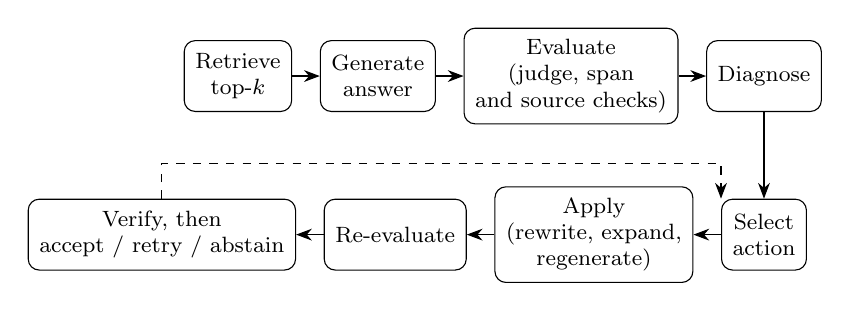
\begin{tikzpicture}[
  node distance=0.55cm and 0.35cm,
  box/.style={draw, rounded corners, align=center, font=\footnotesize\sffamily,
              minimum height=0.9cm, inner sep=4pt},
  arr/.style={-{Stealth[length=2mm]}}]
\node[box] (ret) {Retrieve\\top-$k$};
\node[box, right=of ret] (gen) {Generate\\answer};
\node[box, right=of gen] (judge) {Evaluate\\(judge, span\\and source checks)};
\node[box, right=of judge] (diag) {Diagnose};
\node[box, below=1.1cm of diag] (sel) {Select\\action};
\node[box, left=of sel] (apply) {Apply\\(rewrite, expand,\\regenerate)};
\node[box, left=of apply] (rejudge) {Re-evaluate};
\node[box, left=of rejudge] (ver) {Verify, then\\accept / retry / abstain};
\draw[arr] (ret) -- (gen);
\draw[arr] (gen) -- (judge);
\draw[arr] (judge) -- (diag);
\draw[arr] (diag) -- (sel);
\draw[arr] (sel) -- (apply);
\draw[arr] (apply) -- (rejudge);
\draw[arr] (rejudge) -- (ver);
\draw[arr, dashed] (ver.north) -- ++(0,0.45) -| (sel.north west);
\end{tikzpicture}
\caption{One query through the evaluation-guided loop. The dashed arrow is
a retry while the recovery budget remains.}
\label{fig:loop}
\end{figure}

\section{Using GroundLoop}

An operator builds the system by uploading its documents and specifying its
instructions, chat model, retrieval depth, and recovery policy on the
Configuration page. The Test Console (Figure~\ref{fig:console}) is used for
asking questions. There are four run modes:
\begin{itemize}
\item \textbf{Retrieve only} requires no API key and just shows the passages
  that would be retrieved
\item \textbf{Baseline} produces an answer once
\item \textbf{Confirm recovery} pauses after the diagnosis step and requires
  confirmation before proceeding
\item \textbf{Auto recovery} runs the entire loop
\end{itemize}
Each stage of the loop is lit and timed during a run, and evidence passages
are listed in the evidence panel with their similarity score.

\begin{figure}[htbp]
\centering
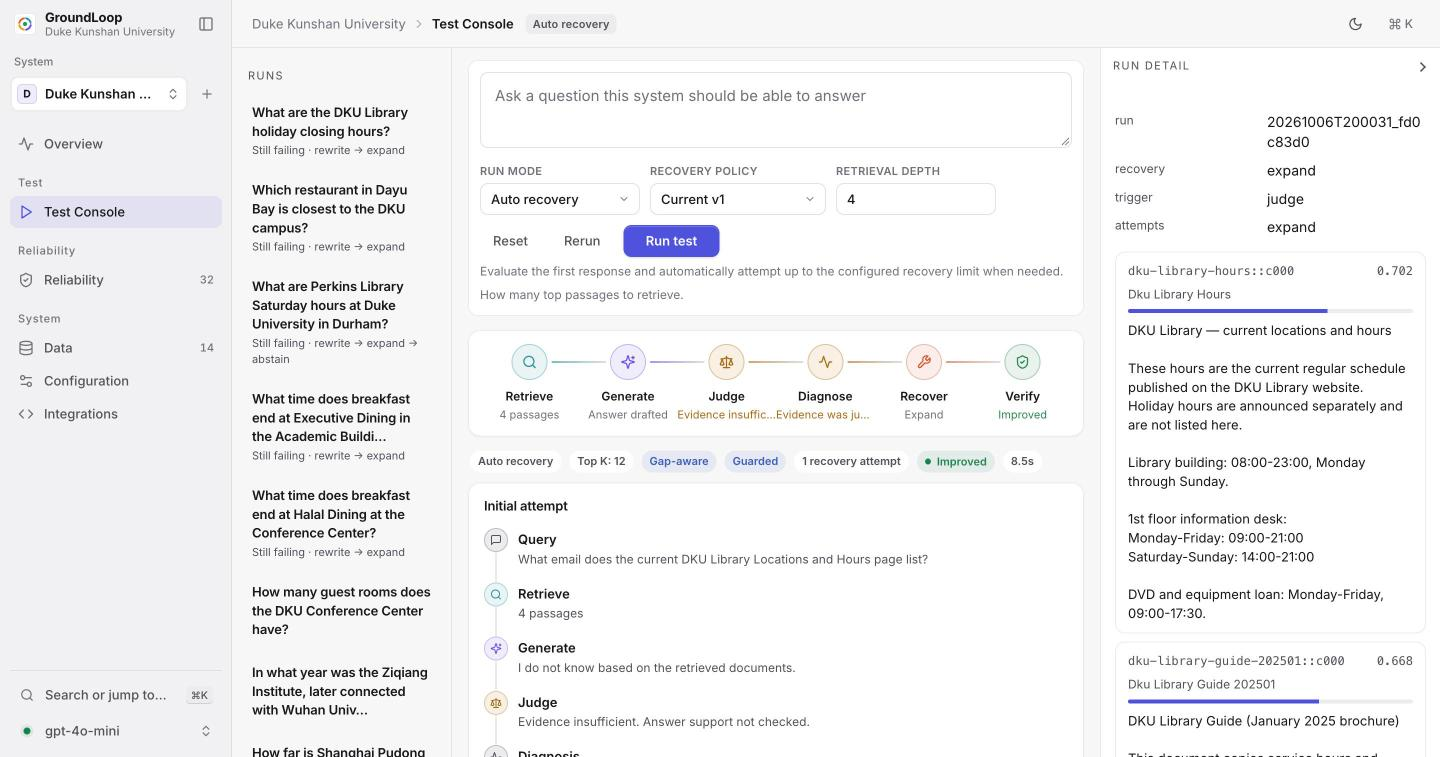
\includegraphics[width=0.85\textwidth]{figures/test-console.jpg}
\caption{The Test Console after an automatic recovery. The loop strip shows
the stage results, and the right panel lists the retrieved passages with
their scores.}
\label{fig:console}
\end{figure}

Each run is saved and can be reviewed later on the Reliability page;
Figure~\ref{fig:answers} shows an example. The first answer is ``I do not
know'' because the required passage was not retrieved. The judge found
the evidence insufficient, and so the loop expanded retrieval from 4 to 12
passages. The answer now shows the email address of the library, with a
citation to the passage it used. The verification box states what the
verdict means and does not mean.

\begin{figure}[htbp]
\centering
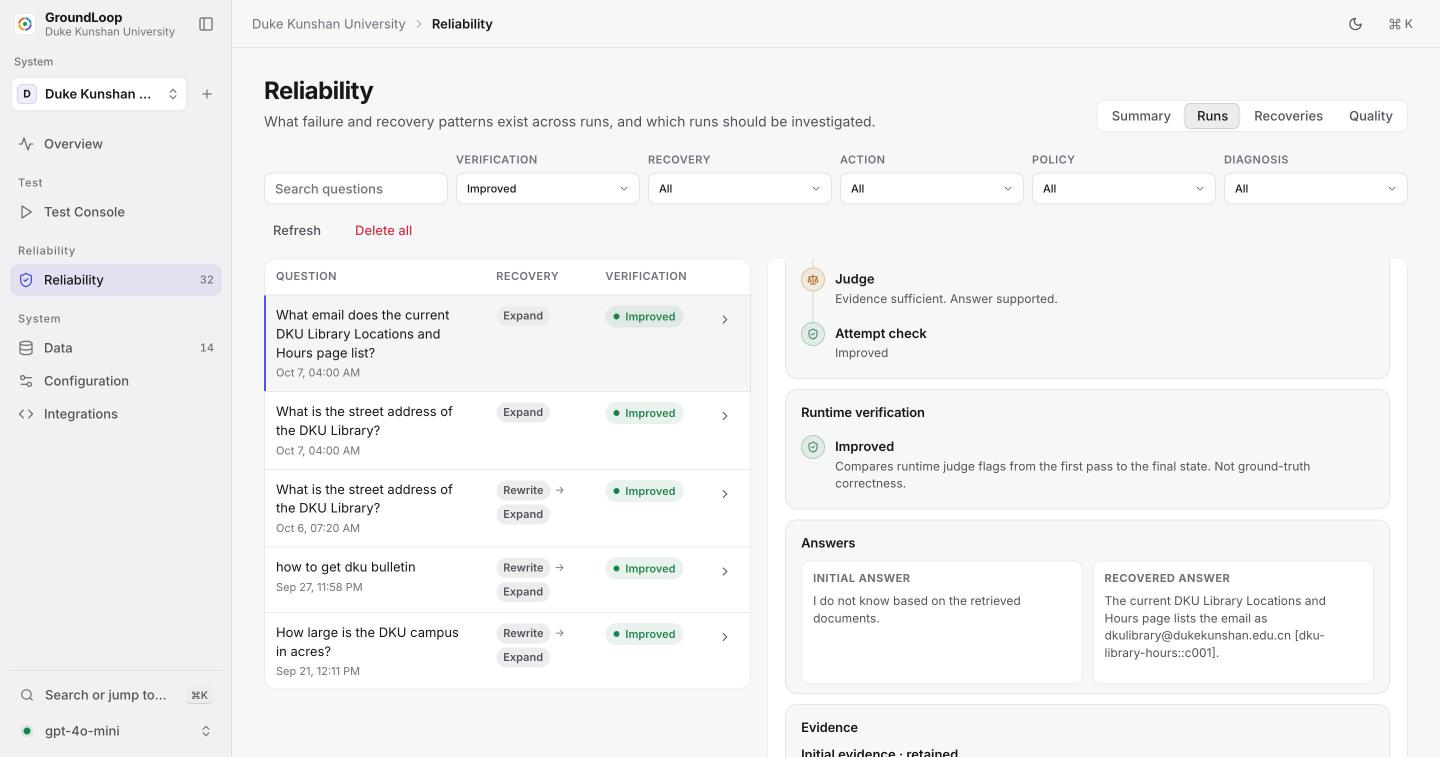
\includegraphics[width=0.85\textwidth]{figures/run-answers.jpg}
\caption{A recovered run in the Reliability view, with the runtime verdict
and the initial and recovered answers side by side.}
\label{fig:answers}
\end{figure}

The Reliability summary in Figure~\ref{fig:reliability} tallies the number
of times recovery was needed across all runs of a system, the number of
diagnoses and actions that took place, the distribution of verdicts and the
judge's flags before and after the first pass and final answer. Runs can be
filtered by verdict, action, policy and diagnosis; this is how the cases
mentioned in Chapter~\ref{results} were identified.

\begin{figure}[htbp]
\centering
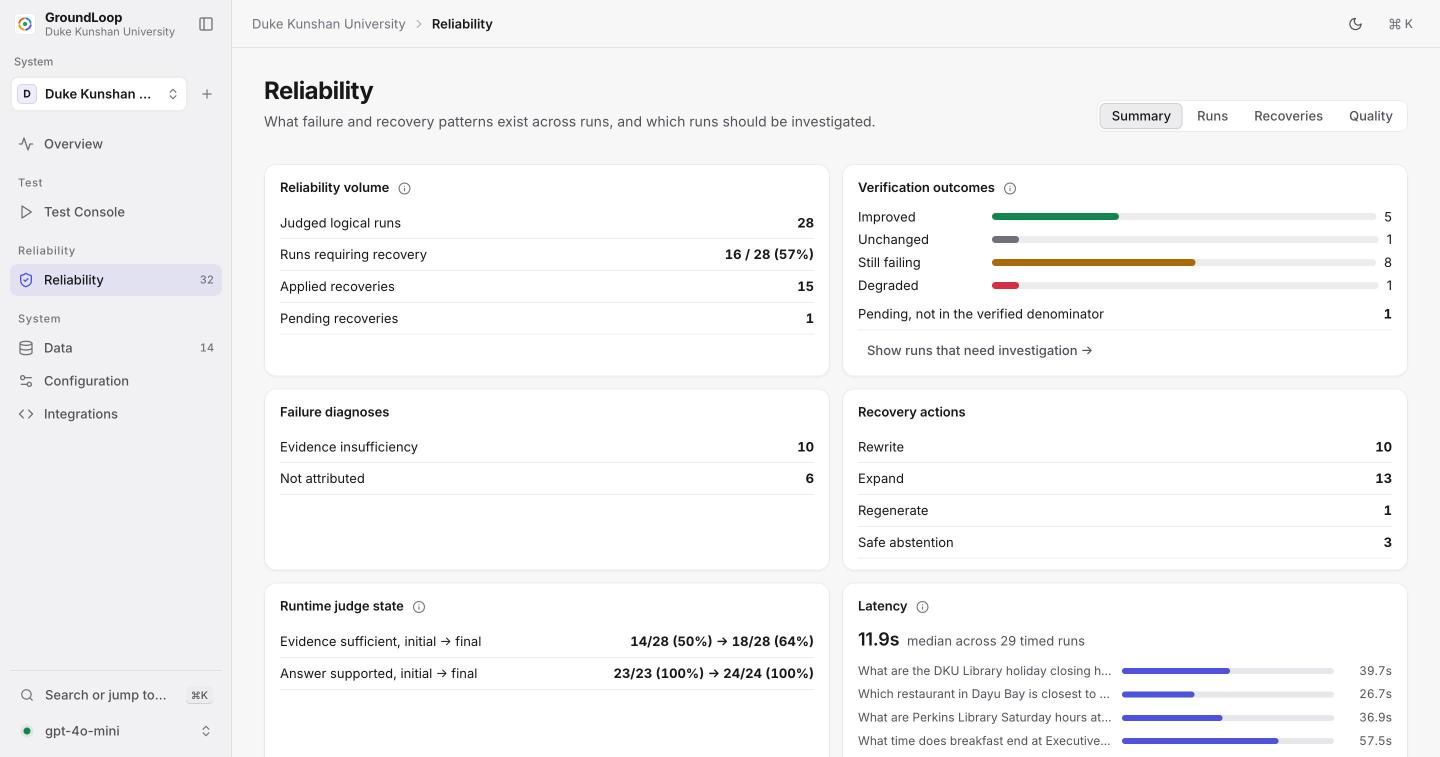
\includegraphics[width=0.85\textwidth]{figures/reliability-summary.jpg}
\caption{The Reliability summary for the Duke Kunshan system.}
\label{fig:reliability}
\end{figure}

An authenticated external API allows an external RAG application to submit
its own question, answer and passages and obtain the judge flags, diagnosis
and suggested recovery. A public demo mode fixes one system in place, does
not allow any changes, and limits runs to a certain number per day.

\section{Design Decisions}

Several decisions influenced the product. They are all tracked in
architecture decision records in the repo and the alternatives explored are
documented.
\begin{itemize}
\item \textbf{A plain web page instead of a framework.} Using a FastAPI
  adapter for static files stayed in one language and didn't require a
  build step. Streamlit would have mixed pipeline code with interface code,
  and using React would have added another toolchain.
\item \textbf{In-memory retrieval.} Using cosine similarity over local files
  was sufficient for dozens of documents, and all the rankings were
  inspectable.
\item \textbf{Single hop retrieval.} Diagnosis becomes unreliable beyond
  single-hop retrieval chains, and the metrics of the project rely on the
  diagnosis being checkable.
\item \textbf{Bounded recovery, safe abstention, operator control.} The loop
  has a bounded budget of actions, doesn't repeat any actions, and abstains
  instead of keeping an answer if its checks are rejected. Confirm mode is
  provided because having a wrong automatic repair is worse than a pause.
\end{itemize}

\section{Engineering and Quality}

The software was developed in small pull requests reviewed thoroughly
before merging, each assigned to an issue, and runs under continuous
integration with Python 3.11 and 3.12 and Node 20. It contains 473 automated
Python tests and 59 JavaScript tests, which use scripted model stand-ins and
thus require no API key. I performed an end-to-end audit of the backend in
October 2026. Four separate reviews and live reruns uncovered 19 issues,
including one scorer that incorrectly scored correct clock ranges, one
rewrite that could end up ``improved'' with an unsupported answer, and one
request that could freeze a benchmark for ten minutes; each issue was fixed
with a test that failed before the fix. Two additional issues, the planted
document masquerading as a passage and the false fix in
Section~\ref{sec:verify}, now have deterministic guards in place.

%%%%%%%%%%%%%%%%%%%%%%%%%%%%%%%%%%%%%%%%%%%%%%%%%%%%%%%%%%%%%%%%

\chapter{Evaluation Method}
\label{material-and-methods}

This chapter describes how the loop inside GroundLoop was measured. The
study runs used the same engine as the console, in automatic mode.

\section{Models and Collections}

\code{gpt-4o-mini} with temperature~0 is used for generation, judging,
regeneration, and query rewriting. Passages are embedded with
\code{text-embedding-3-small}. The same chat model is used for generator
and judge. Documents are split into chunks of at most 500 characters with
80 character overlap. A query retrieves the $k$ closest chunks by cosine
similarity.

Each prompt that takes retrieved text takes each chunk wrapped in a tag
that denotes its id, escapes any occurrence of a tag present in a document,
and declares that the chunk text is data and never part of instructions. A
citation to a chunk that the model was not shown is removed from its
answer. These changes were made after reviewing an answer where a chunk
header that had been planted was indistinguishable from a real header.

Each collection consists of plain text documents and a gold question set.
Each gold row contains a question string, an answerability label, accepted
answer string(s), and supporting document strings. Questions are asked that
are known to be unanswerable, so that abstentions can be scored. The three
study collections are summarized in Table~\ref{tbl:corpora}. The documents
contain superseded notices, near-duplicates of facilities, and facts denied
in the documents.

\begin{table}[htbp]
\centering
\footnotesize
\setlength{\tabcolsep}{5pt}
\begin{tabular}{@{}lllrrr@{}}
\toprule
Collection & Domain & Source & Files & Answerable & Not answerable \\
\midrule
Harbor Institute & Research campus & Fictional & 11 & 23 & 9 \\
Duke Kunshan University & University campus & Public facts & 14 & 30 & 10 \\
Kestrel Aero Components & Aerospace parts & Fictional & 16 & 12 & 4 \\
\bottomrule
\end{tabular}
\caption{Study collections and gold question counts.}
\label{tbl:corpora}
\end{table}

I signed off each gold row on 11 October 2026. An audit of the scorer and
gold set on 15 and 16 October resulted in four changes, each with reason
recorded. Harbor \code{seed-007} (``which shuttle stop is closest to the
boat museum?'') was relabeled to answerable because the shuttle document
states that Library Plaza is the stop to walk to; Harbor has 23 answerable
and 9 unanswerable questions. An answer that correctly rejects the false
premise of an unanswerable question (``the Annex has no group rooms'') now
counts as an abstention, using accepted rejection phrases if they are listed
for the question. An answer that states a near-neighbor's fact counts as an
attempt even if it hedges. Clock ranges are compared as two times. Common
refusal wordings count as abstentions. These changes were made after a
large number of answers had already been generated. The earlier
single-depth runs, rescored under these changes, are available in
Table~\ref{tbl:rescored} of Appendix~\ref{appendix-a}.

\section{Evaluation, Recovery, and Verification}

The grounding judge takes question, the retrieved chunks, and the answer,
and outputs two signals indicating whether the evidence would answer the
question, and whether each fact mentioned in the answer appears in the
evidence. The model does not have access to outside knowledge, does not
count fluency as support, and never sees gold. These two checks can override
the supported label:
\begin{itemize}
\item \textbf{Span check:} The check extracts clock times, emails, ordinals,
  specification tokens, and numbers of three or more digits. If any of these spans
  are missing in the retrieved text, the answer is rejected.
\item \textbf{Source check:} If a question is of the form ``what does [source] say
  about...'', and the answer cites a different source without mentioning
  what the source being asked says, then the answer is not supported.
\end{itemize}

A computed retrieval signal marks a hit as weak if the top score is less
than $0.15$ or $(s_1-s_2)/s_1$ is less than $0.02$; these values were chosen
by hand.

An answer marked unsupported on the first pass and with enough evidence
becomes \emph{unsupported generation}. Insufficient evidence is only
assigned after a second retrieval, becoming a \emph{retrieval miss} if
evidence would have been sufficient or \emph{evidence insufficiency} if
not. This is the default recovery policy. The study budget is two
recoveries, and later action never repeats an earlier one. Any final expand
or regenerate that still fails a check or lacks evidence becomes an
abstention, which does not count as an action from the budget, nor does an
expand that cannot further expand retrieval.

\begin{table}[htbp]
\centering
\small
\begin{tabular}{@{}p{4.4cm}p{2.2cm}p{7.2cm}@{}}
\toprule
State & Action & Effect \\
\midrule
Unsupported generation & Regenerate & New answer from the same chunks. \\
Evidence insufficient (first pass) & Rewrite & New query; answer again only
if the new evidence is sufficient. \\
Judge accepts, retrieval signal weak & Expand & Same query, wider $k$
($1$ or $2 \to 8$, $4 \to 12$, cap 20). \\
Evidence insufficient after rewrite & Abstain & ``I do not know based on
the retrieved documents.'' \\
No failure & Accept & Answer kept. \\
\bottomrule
\end{tabular}
\caption{Default recovery policy.}
\label{tbl:actions}
\end{table}

The verifier compares the old and new flags, and returns \emph{improved},
\emph{degraded}, \emph{still failing}, or \emph{unchanged}. Offline scoring, which
the running system does not see, reports contains-answer for answerable
questions and abstention for unanswerable questions, following SQuAD~2.0 in
treating an abstention for an unanswerable question as
correct~\cite{rajpurkar2018squad}. It also assigns a gold failure class for
the baseline's answer to each question, \emph{no failure} if it was correct,
\emph{evidence insufficiency} if the question is unanswerable,
\emph{retrieval miss} if no document was retrieved that supported the
question, and \emph{unsupported generation} if one was retrieved but the
answer was wrong or abstained. Exact match is near zero because answers are
sentences and gold spans are short, so contains-answer is the quality
metric.

Agreement with gold is measured in two ways:
\begin{itemize}
\item \textbf{F1 sign.} The runtime agrees with the gold when it has the
  same direction as F1.
\item \textbf{Rank rule.} Each answer is either correct, abstained on an
  answerable question, or wrong. The runtime agrees with the gold when it
  has the same transition in ranks. Paraphrases within a rank do not count
  as a transition.
\end{itemize}
The rank rule considers an abstention continued on an unanswerable question
to be \emph{unchanged} (it was correct both times). The runtime considers it
still a failure (the evidence is still missing). This cell is separately
annotated.

\section{Study Design}

Each full gold set for a collection is run once per repeat under seven
conditions, in order: the retrieve-once baseline and the loop at $k=1$, $2$,
and $4$, and a plain baseline at $k=8$. Lower $k$ causes the first pass to
miss more often, providing something for recovery to fix. The $k=8$
baseline tests whether simply fetching more is better than the loop at
lower cost, since the loop's own expand step fetches 8 or 12. Each set of
conditions is run three times on the same code (repository commit
\code{b125064}), and the tables show mean and range. Each run's conditions
are consecutive, and latencies are comparable within each collection. Cost
is an estimate from list price (\$0.15 and \$0.60 per million input and
output tokens), not an invoice. The judge audit is the same as the previous
study: 40 judge calls were sampled with a fixed seed, 20 of the 20
first-pass calls that triggered on recovery and set the support flag, and 20
accepted final calls; the labeler only saw the question, evidence, and
answer, and the same two flags; the labels were reviewed after a previous AI
labeling pass, and are not an independent blind rating.

%%%%%%%%%%%%%%%%%%%%%%%%%%%%%%%%%%%%%%%%%%%%%%%%%%%%%%%%%%%%%%%%

\chapter{Results}
\label{results}

{\raggedright All numbers come from committed result folders. The sweep is
in \texttt{experiments/results/20261015-v5-*} and is summarized by
\texttt{scripts/summarize\_sweep.py} in
\texttt{experiments/rescored/v5-sweep-20261015/}.\par}
Each figure is the mean of three repeats; no significance test is applied.
A provider timeout removed \code{dku-020} from one Duke Kunshan run.

\section{Answer Quality Across Retrieval Depth}

Table~\ref{tbl:sweep} shows the ratio of answerable questions with a gold
span in the answer, and the ratio of unanswerable questions on which the
system abstained or correctly rejected the premise.

\begin{table}[htbp]
\centering
\footnotesize
\setlength{\tabcolsep}{4pt}
\begin{tabular}{@{}llrrrrrr@{}}
\toprule
 & & \multicolumn{2}{c}{Harbor} & \multicolumn{2}{c}{Duke Kunshan} & \multicolumn{2}{c}{Kestrel} \\
\cmidrule(lr){3-4}\cmidrule(lr){5-6}\cmidrule(l){7-8}
Condition & $k$ & Contains & Abstains & Contains & Abstains & Contains & Abstains \\
\midrule
Baseline & 1 & 0.870 & 0.778 & 0.809 & 1.000 & 0.917 & 1.000 \\
Loop     & 1 & 1.000 & 0.741 & 0.966 & 0.967 & 1.000 & 1.000 \\
Baseline & 2 & 0.913 & 0.667 & 0.933 & 0.967 & 1.000 & 1.000 \\
Loop     & 2 & 0.986 & 0.741 & 1.000 & 1.000 & 1.000 & 1.000 \\
Baseline & 4 & 1.000 & 0.778 & 0.966 & 0.967 & 1.000 & 1.000 \\
Loop     & 4 & 1.000 & 0.889 & 1.000 & 0.933 & 1.000 & 1.000 \\
Baseline & 8 & 1.000 & 0.852 & 1.000 & 1.000 & 1.000 & 1.000 \\
\bottomrule
\end{tabular}
\caption{Contains-answer rate on answerable questions, and abstention rate
on unanswerable questions. Mean of three repeats. Harbor has 23 answerable
and 9 unanswerable questions, Duke Kunshan 30 and 10, Kestrel 12 and 4.}
\label{tbl:sweep}
\end{table}

At $k=1$ the loop increased the contains-answer rate on all three corpora:
Harbor from 0.870 to 1.000, Duke Kunshan from 0.809 to 0.966, Kestrel from
0.917 to 1.000. At $k=2$ the increases were smaller and at $k=4$ the
baseline was already at or near 1.000. The plain baseline reached 1.000 on
all three corpora at $k=8$. Abstention changed by at most one question in
either direction, except on Harbor at $k=4$, where the loop abstained on 8
of 9 unanswerable questions compared to the baseline's 7.

Contains-answer for a condition varied by at most one question between
repeats.

\begin{table}[htbp]
\centering
\footnotesize
\begin{tabular}{@{}lllll@{}}
\toprule
Collection & & $k=1$ & $k=2$ & $k=4$ \\
\midrule
Harbor & fixed & 3, 3, 3 & 3, 3, 3 & 1, 1, 1 \\
       & broke & 0, 1, 0 & 1, 1, 0 & 0, 0, 0 \\
Duke Kunshan & fixed & 5, 5, 4 & 3, 2, 2 & 1, 1, 2 \\
             & broke & 0, 1, 0 & 0, 0, 0 & 1, 0, 1 \\
Kestrel & fixed & 1, 1, 1 & 0, 0, 0 & 0, 0, 0 \\
        & broke & 0, 0, 0 & 0, 0, 0 & 0, 0, 0 \\
\bottomrule
\end{tabular}
\caption{Questions fixed and broken by the loop compared to the baseline
(same depth).}
\label{tbl:fixbreak}
\end{table}

Fixed and broke counts over 27 loop runs (three depths, three collections,
three repeats) are fixed 49, broke 6. I've read all six. Five are
unanswerable questions that the loop correctly rejected without the
rejection list containing the rejection's words (e.g.\ ``breakfast is not
served there'' for \code{dku-032}). One is a genuine regression: Harbor
\code{seed-007} $k=2$, the loop abstained while the baseline was correct.

The gold decisions made after seeing answers do not drive this pattern.
Scored with the gold set as it stood on 11 October, contains-answer at
$k=1$ still rises from 0.864 to 1.000 on Harbor and from 0.809 to 0.966 on
Duke Kunshan, and the $k=8$ baseline still reaches 1.000 on both. Only the
abstention rates fall, because correct premise rejections are not credited.

\section{Runtime Diagnosis}

Table~\ref{tbl:diagnosis} shows the comparison between the loop's diagnosis
at $k=1$ and the gold failure class pooled across nine runs.

\begin{table}[htbp]
\centering
\footnotesize
\begin{tabular}{@{}lrl@{}}
\toprule
Gold class & Questions & Loop's diagnosis \\
\midrule
No failure & 165 & left alone 163, retrieval miss 2 \\
Evidence insufficiency & 69 & evidence insufficiency 62, none 7 \\
Retrieval miss & 17 & retrieval miss 14, none 3 \\
Unsupported generation & 12 & retrieval miss 12 \\
\bottomrule
\end{tabular}
\caption{Loop diagnosis vs.\ the gold failure class. $k=1$, nine runs.}
\label{tbl:diagnosis}
\end{table}

The loop left 163 of 165 correct answers unchanged, labeled 62 of 69
unanswerable questions as evidence insufficiency, and correctly labeled 14
of 17 retrieval misses. The loop never made an unsupported generation
diagnosis. All 12 such cases are four questions (\code{dku-012},
\code{dku-013}, \code{gold-015}, \code{gold-024}) and three repeats. In each
repeat the baseline abstained although a supporting document had been
retrieved, the loop diagnosed it as a retrieval miss, expanded retrieval and
answered correctly. When $k=1$, the gold rule counts a document as found even
when the passage with the answer was not, so these disagreements can be said to
arise as much from the gold rule as from the loop.

Because the action follows from the diagnosis (Table~\ref{tbl:actions}),
action suitability shows in Table~\ref{tbl:fixbreak}.

\section{Cost}

Table~\ref{tbl:cost} shows chat calls, estimated cost, and median latency
per run for each collection.

\begin{table}[htbp]
\centering
\footnotesize
\setlength{\tabcolsep}{4pt}
\begin{tabular}{@{}llrrrrrrrrr@{}}
\toprule
 & & \multicolumn{3}{c}{Harbor} & \multicolumn{3}{c}{Duke Kunshan} & \multicolumn{3}{c}{Kestrel} \\
\cmidrule(lr){3-5}\cmidrule(lr){6-8}\cmidrule(l){9-11}
Condition & $k$ & Calls & USD & s & Calls & USD & s & Calls & USD & s \\
\midrule
Baseline & 1 & 32 & 0.0018 & 4.6 & 40 & 0.0022 & 5.0 & 16 & 0.0007 & 4.8 \\
Loop     & 1 & 107 & 0.0127 & 10.9 & 140 & 0.0170 & 13.0 & 52 & 0.0051 & 11.4 \\
Baseline & 2 & 32 & 0.0025 & 4.9 & 40 & 0.0031 & 4.6 & 16 & 0.0009 & 5.5 \\
Loop     & 2 & 111 & 0.0153 & 10.9 & 129 & 0.0178 & 9.3 & 48 & 0.0051 & 10.3 \\
Baseline & 4 & 32 & 0.0036 & 4.8 & 40 & 0.0045 & 4.3 & 16 & 0.0013 & 5.5 \\
Loop     & 4 & 107 & 0.0190 & 9.3 & 129 & 0.0235 & 10.2 & 48 & 0.0064 & 11.0 \\
Baseline & 8 & 32 & 0.0060 & 4.6 & 40 & 0.0073 & 3.7 & 16 & 0.0020 & 4.9 \\
\bottomrule
\end{tabular}
\caption{Chat calls per run, estimated cost per run (in US dollars), and
median latency per question (in seconds). Mean across three repeats.}
\label{tbl:cost}
\end{table}

The loop made 3.0-3.5x as many chat calls as the same-depth baseline and
took 1.9-2.6x as long to answer each question. Since the expansion strategy
also passes more passages to the model, it cost 4.9-7.7x as much as the
same-depth baseline. The $k=8$ baseline cost 39-47 percent of the loop at $k=1$ and
matched or exceeded its contains-answer rate on every collection. The full
sweep (9 runs across 7 conditions) cost roughly \$0.47.

\section{Runtime Verification}
\label{sec:verify}

Table~\ref{tbl:verify} compares each runtime verdict with the gold rank
transition, pooled over repeats and depths.

\begin{table}[htbp]
\centering
\footnotesize
\begin{tabular}{@{}lrrrr@{}}
\toprule
 & \multicolumn{2}{c}{Answerable} & \multicolumn{2}{c}{Unanswerable} \\
\cmidrule(lr){2-3}\cmidrule(l){4-5}
Collection & Verified & Agrees & Verified & Agrees \\
\midrule
Harbor & 29 & 21 & 71 & 1 \\
Duke Kunshan & 41 & 35 & 90 & 0 \\
Kestrel & 3 & 3 & 36 & 0 \\
\midrule
Total & 73 & 59 & 197 & 1 \\
\bottomrule
\end{tabular}
\caption{Runtime verdict against the gold rank transition, all loop runs.}
\label{tbl:verify}
\end{table}

On answerable questions the verdict matched gold on 59 of 73 recovered
runs. On unanswerable ones it matched 1 of 197, but almost all are a kept
abstention that the runtime calls \emph{still failing} and the rank rule
\emph{unchanged}: a difference in vocabulary, not a wrong decision.

One case was a wrong answer. How long did the 1948 gale last according
to the Coastal Memory Group, Harbor \code{gold-029} asks; that group holds
nothing after 1940. The answer included a 19 hours
figure from another archive, which the source check rejected. In one repeat
the 19 hours was attributed to the Coastal Memory Group, which the judge
accepted and the verifier judged an improvement. After the sweep a further
check was added to make such figures appear in the relevant passages in the
source cited; out of 1{,}164 answers stored it triggers only in this answer.

The 40 judge calls were audited separately. For the sufficiency flags the
judge agreed with the human ratings on 39 answers; for the support flags on
39. The ratings are not independent blind ratings; the two disagreements were cases
where the answer used a figure from another archive (the judge agreed) and
a correct ``the collection does not say'' answer (the judge said
unsupported).

%%%%%%%%%%%%%%%%%%%%%%%%%%%%%%%%%%%%%%%%%%%%%%%%%%%%%%%%%%%%%%%%

\chapter{Discussion}
\label{discussion}

\section{When Recovery Helps}

Sweep distinguishes two cases neither of which could be meaningfully
analyzed in the previous study. When the first query return is sparse
($k=1$ or $2$), the loop corrected almost everything the baseline could not;
49 questions repaired against 1 real regression, the same across all three corpora, and
independent of the repeats. When the first query return contains the answer
($k=4$), there was little to correct, and the loop's impact was reduced to
one question per run. The finding that the loop ``barely moves accuracy'' in
the previous study was due to the particular conditions under which it was
tested. The corrections derived mostly from expansion: the correction the
loop is designed to make here is a retrieval failure, which explains the
role of the 8 baseline.

\section{Against a Simpler Alternative}

Retrieving eight passages from the start reaches the loop's best
contain-answer rate on each collection at under half the cost of the loop
(in tokens) at $k=1$ and under half the time. On these collections, the
wider baseline configuration matches the quality of the loop at lower cost.
What the loop buys over the narrower baseline that the wider baseline does
not is a record of a diagnosis, an action, and a verdict for every question
it looked at. On larger collections, where eight passages is more expensive
or long context hurts the generator~\cite{liu2024lost}, the balance could
flip; these runs are not indicative of that.

\section{Verification and the Judge}

For answerable questions, the runtime verdict agreed with the gold's rank
transition in 59 out of 73 runs recovered. This is a stronger test than the
previous F1-sign figure since the sweep actually made repairs that the
verdict could see. The unanswerable cell is just a naming issue and should
be reported separately.

The source switch in \code{gold-029} is the most egregious issue in this
project. The loop responded to a rejection by changing the source it named, the judge
accepted the outcome, and the verifier reported a repair. This is the risk
of loops which can game their own feedback to satisfy it without answering
the question~\cite{huang2024cannot,kamoi2024selfcorrection}. The
deterministic check closes the case. This is just
a single case, and the check was added after witnessing it.

\section{Relation to Prior Work and Limits}

Task accuracies are reported after action in corrective and adaptive RAG
systems~\cite{jiang2023flare,asai2024selfrag,yan2024crag,jeong2024adaptiverag}.
Here recovery helped more when retrieval was starved, and the wider search
matched the improvement in accuracy with more retrieved. Adaptive-RAG
advocates targeted retrieval effort only on questions that needed
it~\cite{jeong2024adaptiverag}. This project explores the balance of the
version of that trade on small datasets and finds the wider, unchanging
retrieval to be cheaper. Like Joren et al., sufficiency drove
abstention~\cite{joren2025sufficient} - the scorer required phrases to
reject premises, and still missed five. Limitations of design and data
constrain the reading of this paper. The model generates and scores,
verification reads two flags, the span and source checks apply to a few
fact types, and the thresholds for retrieval were hand-tuned. Small,
hand-crafted datasets were used and single-hop was assumed. The judge
sample is 40 calls and not independently annotated. The need for recovery
was annotated by one reviewer. There have been no other users of the
console. The gold relabel, the rejection phrases, and the source checks
were informed by the answers. Three repeats use one model at
temperature~0.

%%%%%%%%%%%%%%%%%%%%%%%%%%%%%%%%%%%%%%%%%%%%%%%%%%%%%%%%%%%%%%%%

\chapter{Conclusions}
\label{conclusions}

Evaluation-guided recovery fixed most of the questions that a thin
first-stage retrieval missed on three small single-hop collections. At
$k=1$, it improved `contains-answer' from 0.81 to 0.97 on Duke Kunshan and
to 1.00 on Harbor and Kestrel (one actual regression out of 27 loop
runs). It made almost no repairs when the initial retrieval was sufficient. In all
experiments it made about three times as many chat calls as the same-depth
baseline (taking about twice as long). A plain baseline that retrieved
eight passages matched the loop's quality at less than half the cost.

The loop's self-assessment was more accurate than could be shown in the
previous study: it diagnosed most failures as the gold did (76 out of 98),
and its verdict matched the gold verdict in 59 out of 73 answerable
recoveries. It made one confident false repair (the answer kept a wrong
number, changing only the source cited). The program reveals the diagnosis,
action, and verdict called for by the ChatDKU gap question. On these
collections, they explain what the loop did. A recovery verdict is evidence
that can be inspected, not proof that a repair was made, and a better wider
retrieval is what any claim for the loop has to beat.

\section{Future Work}

I want to make GroundLoop into a product that other teams can use and pay
for. The most straightforward way to do this is as a layer on top of an
existing RAG setup: developers continue to own their own retriever and
model, and sends each question, answer, and passages to our evaluation API,
and receives a diagnosis, recovery, verdict, and each run is traced and can
be viewed by the developer. Three things that this project didn't have that
I need to get here are testing with external users to shape the console and
API by people who did not build them, evaluation on larger question sets written by
others, with more than one model and including multi-hop questions, and an
ablation to show whether diagnosis is necessary, or just broadening
retrieval when the judge complains. The $k=8$ result is as much a product
question as a research question: GroundLoop needs to justify its cost in
explanations, not just its accuracy.

%%%%%%%%%%%%%%%%%%%%%%%%%%%%%%%%%%%%%%%%%%%%%%%%%%%%%%%%%%%%%%%%

\chapter*{References}
\label{references}
\addcontentsline{toc}{chapter}{References}


\instructions{Many bibliographic styles are acceptable for publications in the natural sciences. This template uses a numeric style defined in biblatex and that is common in Physics, Mathematics, and Computer Science papers.}

\printbibliography[heading=none]


%%%%%%%%%%%%%%%%%%%%%%%%%%%%%%%%%%%%%%%%%%%%%%%%%%%%%%%%%%%%%%%%

\chapter*{Signature Work Narrative}
\label{narrative}
\addcontentsline{toc}{chapter}{Signature Work Narrative}

When I came to Duke Kunshan University, I knew that I wanted to work in technology and be a software engineer. I am an Applied Math and Computational Science major with a track in Computer Science. As I went through DKU, I realized my interests became more specific. Technology was also rapidly changing during my time at DKU, especially with the rise of artificial intelligence and large language models. As I learned more through classes, research, internships, and personal projects, AI is the type of technology I am the most interested in.

The primary motivation for my Signature Work came from my research experience at DKU. I had my first taste of AI research with Professor Paul Weng. I did a few different tasks, but I eventually focused more on evaluation. This was where I started thinking about AI research where not only do you have to build the AI system, but you also need to evaluate if the AI system is good or not.

After doing research with Professor Weng over the summer, I started to work with Professor Bing Luo's research group on ChatDKU, a DKU-focused retrieval-augmented generation, or RAG, system. They took me in, and my main role was to work on the evaluation pipeline and evaluate the RAG system.

While doing this, I always had this one question in mind: ``And then what?'' Because with an evaluation, I would get a score telling me how good or bad the system was, but I would always think, ``And then what?'' With the score, I would know something was wrong or right, but I wouldn't know why it happened or what part of the pipeline was faulty or what comes next.

I also attempted to work on automated evaluation while I was with ChatDKU, but I never really finished it because automated evaluation was more complicated than I thought. These questions then led me to my Signature Work. I started to become interested in what more could evaluation do? I wanted to know if evaluation could not only score systems, but it could also diagnose failures and be recoverable or even automated recovery. These questions led me to my Signature Work.

Three classes that really helped lay the foundation to be able to work on this project were MATH 202 - Linear Algebra, CS 101 - Introduction to Computer Science, and CS 201 - Programming and Data Structures. Although I did not take these classes thinking that I would later build an AI reliability system, they helped in different ways.

MATH 202 - Linear Algebra especially became more important to me when I started working with RAG systems. One concept that stood out to me was cosine similarity. Since in RAG systems, you can represent information with embeddings or vectors, you can use cosine similarity to find the similarity between different vectors. While working on evaluation early on, I used cosine similarity a lot when comparing different embeddings and looking at the retrieval performance. Before RAG, vectors and vector similarity was mainly mathematical to me, but through research, I started to realize how these mathematical concepts support modern AI systems. Linear algebra helped me understand more about what was going on inside the retrieval process, rather than looking at the system as a black box.

CS 101 - Introduction to Computer Science helped my Signature Work in a different way. This was my first computer science class, and this class sparked my interest in programming and software engineering. It is not so much the topics, but this class made me realize that programming is something that I want to pursue, and it helped me turn my interest in technology into something that I can actually make. Obviously, GroundLoop is a lot more advanced than what I did in CS 101, but it gave me the problem solving and programming foundation to lead to projects like this.

CS 201 - Programming and Data Structures built off of CS 101 and was more similar to the type of programming I do now. It made me more comfortable with larger programs, data structures, and development environments such as Visual Studio Code. These programs required more organization and structure in how the program was built. This became important to my Signature Work because I did not want GroundLoop to just be a research project or a bunch of scripts. I wanted to build an actual application with an interface, an evaluation pipeline, a trace, and reliability features. CS 201 helped me think about the project not only as research, but also as software.

My capstone experience helped tie all of these academic and research experiences together. Since I was already working with ChatDKU through my capstone experience, I knew that I wanted my Signature Work to come from the problems that I was having with ChatDKU. I asked Professor Bing Luo to be my mentor, and I also worked closely with Mingxi, a PhD student from Wuhan who helped me with my ChatDKU work and my capstone.

The first part of my capstone was very similar to ChatDKU. This gave me the opportunity to work with an actual RAG system and problems in the retrieval, generation, evaluation, and system design. For the second part of my capstone, I focused more on my own Signature Work. ChatDKU then became both the foundation and motivation for GroundLoop.

My project also evolved a lot while I was working on it. Originally, I thought I would use the entire ChatDKU system and data for my Signature Work. However, I quickly realized that the ChatDKU system and context was too complex for the type of question that I wanted to answer. Because with too many things changing at once, it becomes difficult to tell why a recovery or evaluation decision was successful or not. I then decided that I would first work with a more controlled RAG environment so that I can more easily inspect the system.

My literature review also impacted how I viewed my project. Originally, I was interested in the idea of an evaluator detecting a bad answer and triggering recovery automatically. However, I discovered that evaluation guided recovery loops already exist in current research. This made me think about this question in a more interesting way: if an evaluator can trigger recovery, how much can we trust the evaluator?

Instead of taking the evaluator's verdict as gospel, I then became more focused on the reliability of the evaluation and recovery process itself. I started to become interested in questions like was the evaluator accurate in detecting the failure, was the failure recoverable, and does recovery improve the final answer?

I also chose to build GroundLoop as software that people can use rather than just doing a research project. A lot of work in this space is still just in research papers. I saw an opportunity to take these ideas and apply them in a way that developers can use. Rather than trying to compete with existing observability platforms like LangSmith, I became interested in GroundLoop as more of a additional layer of reliability for existing RAG systems.

My project also had results that did not confirm some of my hypotheses. However, this became one of the most valuable parts of my project. In some experiments, recovery helped when retrieval was bad, but just getting more information retrieved can sometimes provide the same improvement at a lower complexity. Earlier on, I would have thought this was a disappointing result because it is not only showing that my system works, but I became more comfortable with the idea that a good result can also mean a simpler solution works just as well. Evaluation should not be about proving that my system works. It is about understanding what the system is doing.

I also used AI coding tools like Claude while developing GroundLoop. My role was still to decide what to build, how to build it, evaluate results, find problems, and make all the key decision making in the project. In some ways, using AI coding tools made evaluation even more relevant to me. Because with software becoming easier to generate, knowing how to test and evaluate the software that is produced is more important than ever.

My Signature Work has also helped me narrow down what I want to do post-DKU. I had a few research experiences at DKU, and I also had internship and software engineering experience. I am thankful for my research experience because it helped me learn how to ask better questions, test hypotheses, and be more careful with what I conclude. It also helped me realize that I prefer the applied side of technology over research itself.

During my internship experience in Shanghai and while building my own software projects, I enjoyed the process of creating things that people could use. Post-DKU, I plan to continue to work as a software engineer and building applications that use AI. I am also interested in pursuing a master's degree, but I am more interested in applied programs that involve computer science, AI, software engineering, and product development rather than a research-focused program.

I also do not necessarily see GroundLoop ending when I submit my Signature Work. One of my goals is to continue developing it as a product and releasing it. I want to see if it becomes something that developers or companies would use and pay for. Regardless of whether or not it becomes a successful company, this project is what I want my career to be: software engineering, AI, evaluation, and product development.

Looking back on my Signature Work, many parts of my experience at DKU led me to where I am now. CS 101 made me want to continue programming. CS 201 made me more comfortable building software. Linear algebra later helped me understand some of the mathematical foundations behind the AI systems that I was evaluating. My research with Professor Paul Weng introduced me to AI evaluation. My work with Professor Bing Luo, Mingxi, and ChatDKU gave me an actual system to work with and see its limitations. My capstone then gave me the opportunity to take those limitations and form my own question and ultimately GroundLoop. Everything came full circle with this experience, showing me that not only do you have to build an AI system, but you also need to understand when it works, why it does not, and what comes next.

%%%%%%%%%%%%%%%%%%%%%%%%%%%%%%%%%%%%%%%%%%%%%%%%%%%%%%%%%%%%%%%%

\appendix

\chapter{Additional Material}
\label{appendix-a}


\instructions{If you have an Overleaf account (either free or paid) you can use this file to start a new Overleaf project.

If you do not want an Overleaf account you can install TeX on your computer and use the template files provided by the Office of Signature Work.}

\section{Software Availability}
\label{sec:availability}

{\raggedright
GroundLoop's source code, tests, benchmark configurations, and every
result folder cited in this paper are kept in a private repository. The
author will grant access to examiners on request.

A read-only snapshot of the GroundLoop console, with recorded Duke Kunshan
runs, can be opened in any browser at
\url{https://sieguerra.github.io/groundloop/} (source:
\url{https://github.com/sieguerra/groundloop}). It shows the interface and
stored traces but does not run new questions.\par}

\section{Study Configurations}

{\raggedright
The depth sweep used \texttt{experiments/configs/v5\_\{harbor,dku,kestrel\}\_depth\_sweep.json}
at repository commit \texttt{b125064}. Its snapshots are
\texttt{experiments/results/20261015-v5-<collection>-r<1,2,3>}, and the
summary is \texttt{experiments/rescored/v5-sweep-20261015/}. The earlier
$k=4$ study is \texttt{20261010T203121} (Harbor), \texttt{20261010T203115}
(Duke Kunshan), and \texttt{20261010T202849} (Kestrel), rescored in
\texttt{experiments/rescored/scoring-v4-gold-2026-10-16/}. Judge-audit files
are in \texttt{experiments/judge-audit/20261011/}. The trace schema is in
\texttt{docs/trace-schema.md}.\par}

\section{Earlier Runs, Rescored}

\begin{table}[htbp]
\centering
\footnotesize
\begin{tabular}{@{}lllll@{}}
\toprule
 & \multicolumn{2}{c}{Contains-answer} & \multicolumn{2}{c}{Unanswerable abstention} \\
\cmidrule(lr){2-3}\cmidrule(l){4-5}
Folder & Stored & Rescored & Stored & Rescored \\
\midrule
Harbor \texttt{20261010T203121} & 0.864 / 0.864 & 1.000 / 1.000 & 0.400 / 0.500 & 0.667 / 0.778 \\
Duke Kunshan \texttt{20261010T203115} & 0.767 / 0.800 & 0.967 / 1.000 & 0.800 / 0.900 & 1.000 / 1.000 \\
Kestrel \texttt{20261010T202849} & 0.917 / 0.917 & 1.000 / 1.000 & 1.000 / 1.000 & 1.000 / 1.000 \\
\bottomrule
\end{tabular}
\caption[Earlier $k=4$ runs, stored and rescored]{Earlier $k=4$ runs, baseline / loop, as stored and as rescored
(\texttt{experiments/rescored/scoring-v4-gold-2026-10-16}).}
\label{tbl:rescored}
\end{table}

\section{Use of AI Tools}

Generative AI tools assisted with this project. They helped write and
review software and run the benchmarks. AI was also used for grammar and
paraphrasing. The research question, design decisions, claims,
interpretation, and conclusions are mine.

\section{Product Tour}

Two further screens complement Figures~\ref{fig:console}
to~\ref{fig:reliability}. The Overview (Figure~\ref{fig:overview}) is the
landing page of a system: it counts how many runs passed through each stage
of the loop and lists the runs that still need attention. The Configuration
page (Figure~\ref{fig:configuration}) shows a system's pipeline and settings
and the four steps for building an editable system on one's own documents.

\begin{figure}[H]
\centering
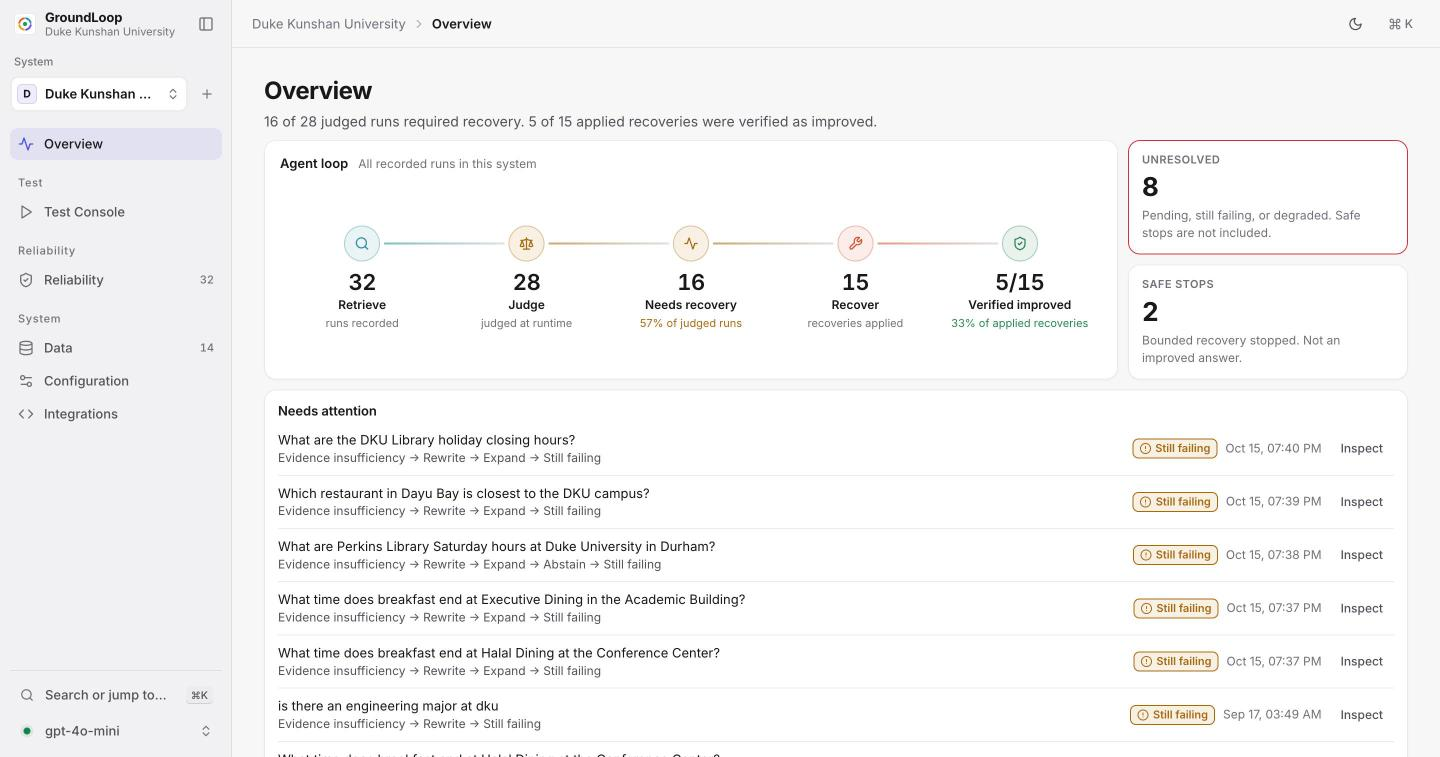
\includegraphics[width=0.8\textwidth]{figures/overview.jpg}
\caption{The Overview page for the Duke Kunshan system.}
\label{fig:overview}
\end{figure}

\begin{figure}[H]
\centering
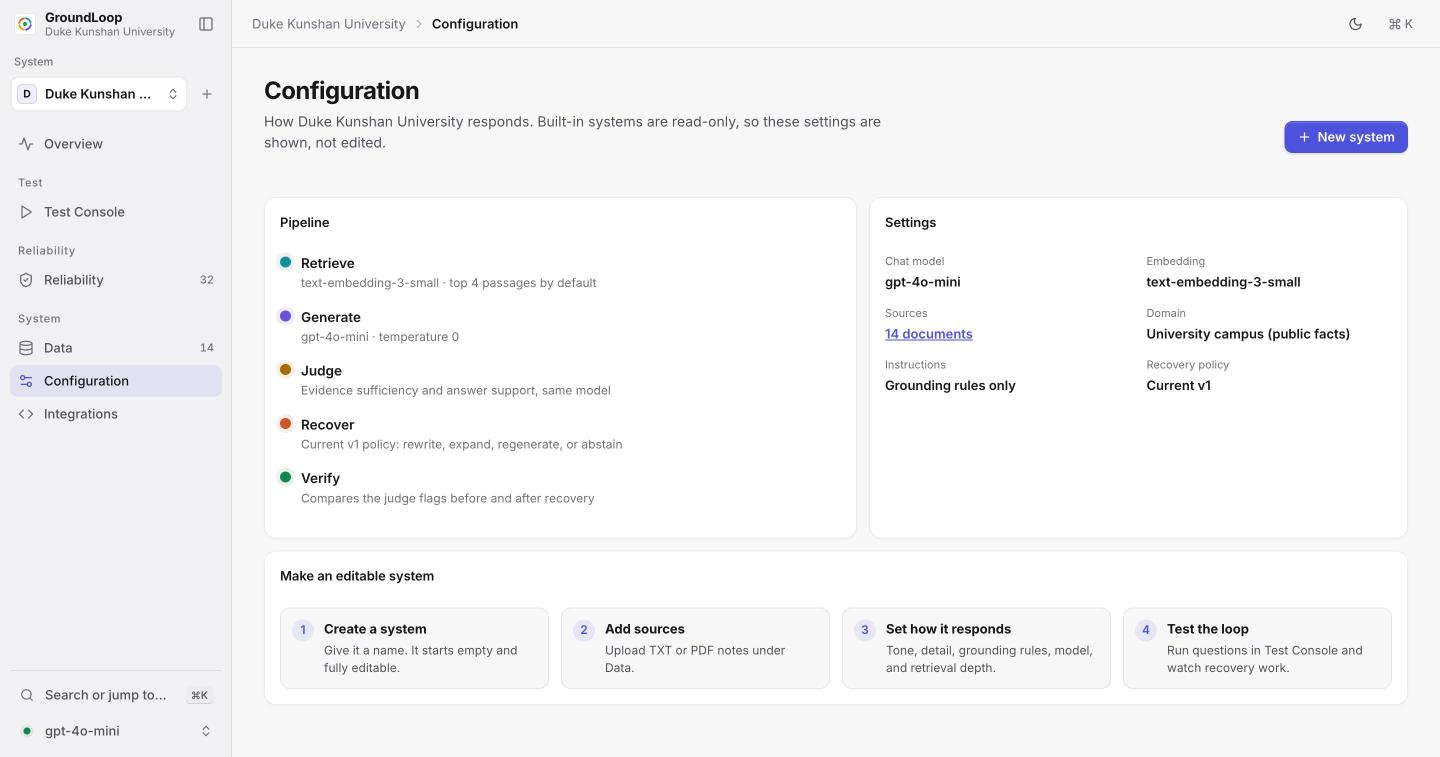
\includegraphics[width=0.8\textwidth]{figures/configuration.jpg}
\caption{The Configuration page. Built-in systems are read-only; a new
system is fully editable.}
\label{fig:configuration}
\end{figure}

Three more screens show the rest of the console. The Runs view of the
Reliability page (Figure~\ref{fig:runs}) lists every run with its recovery
path and verdict; opening a run shows its loop and a timeline of each stage.
The Data page (Figure~\ref{fig:data}) lists a system's source documents and
shows the text of each one. The Integrations page
(Figure~\ref{fig:integrations}) documents the external evaluation API with
examples ready to copy.

\begin{figure}[H]
\centering
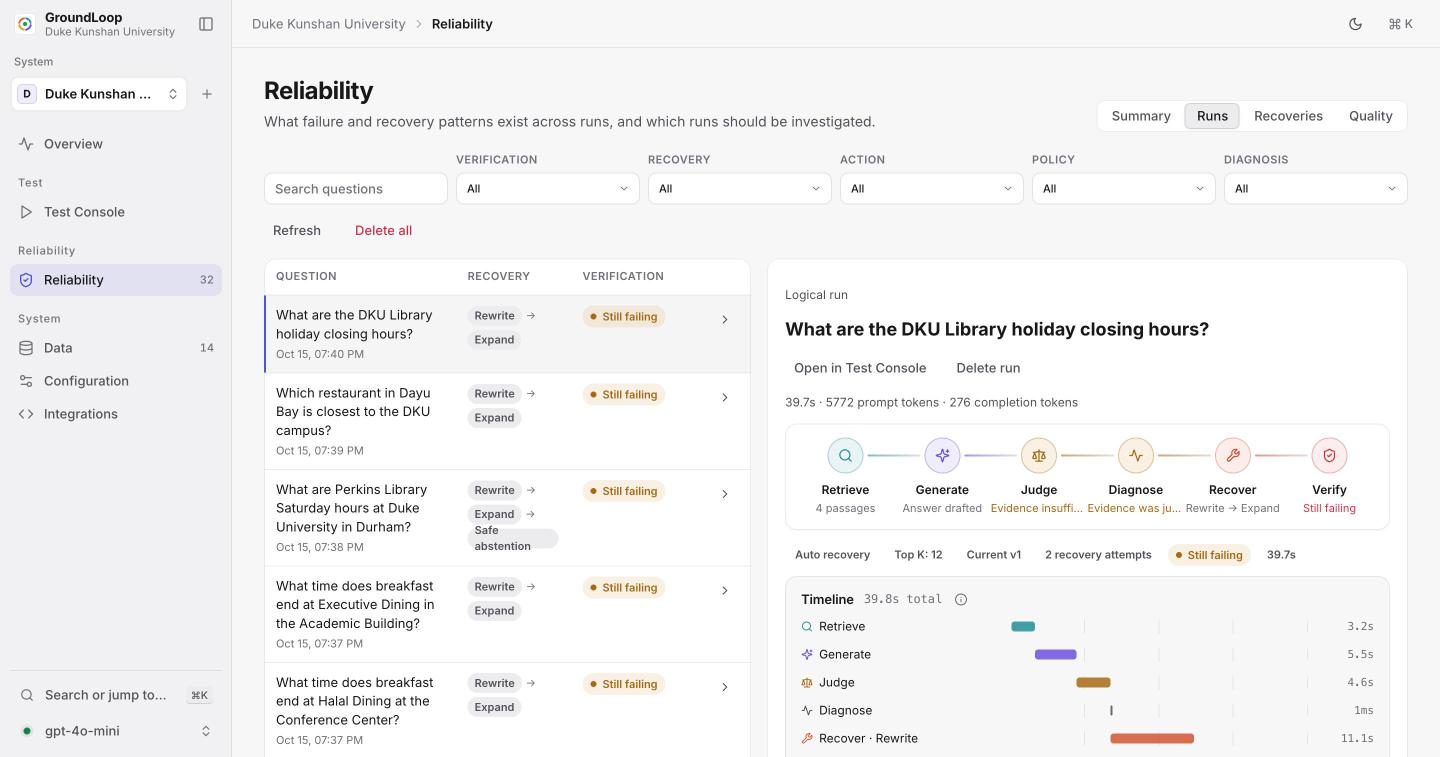
\includegraphics[width=0.8\textwidth]{figures/runs.jpg}
\caption{The Runs view of the Reliability page, with one run opened.}
\label{fig:runs}
\end{figure}

\begin{figure}[H]
\centering
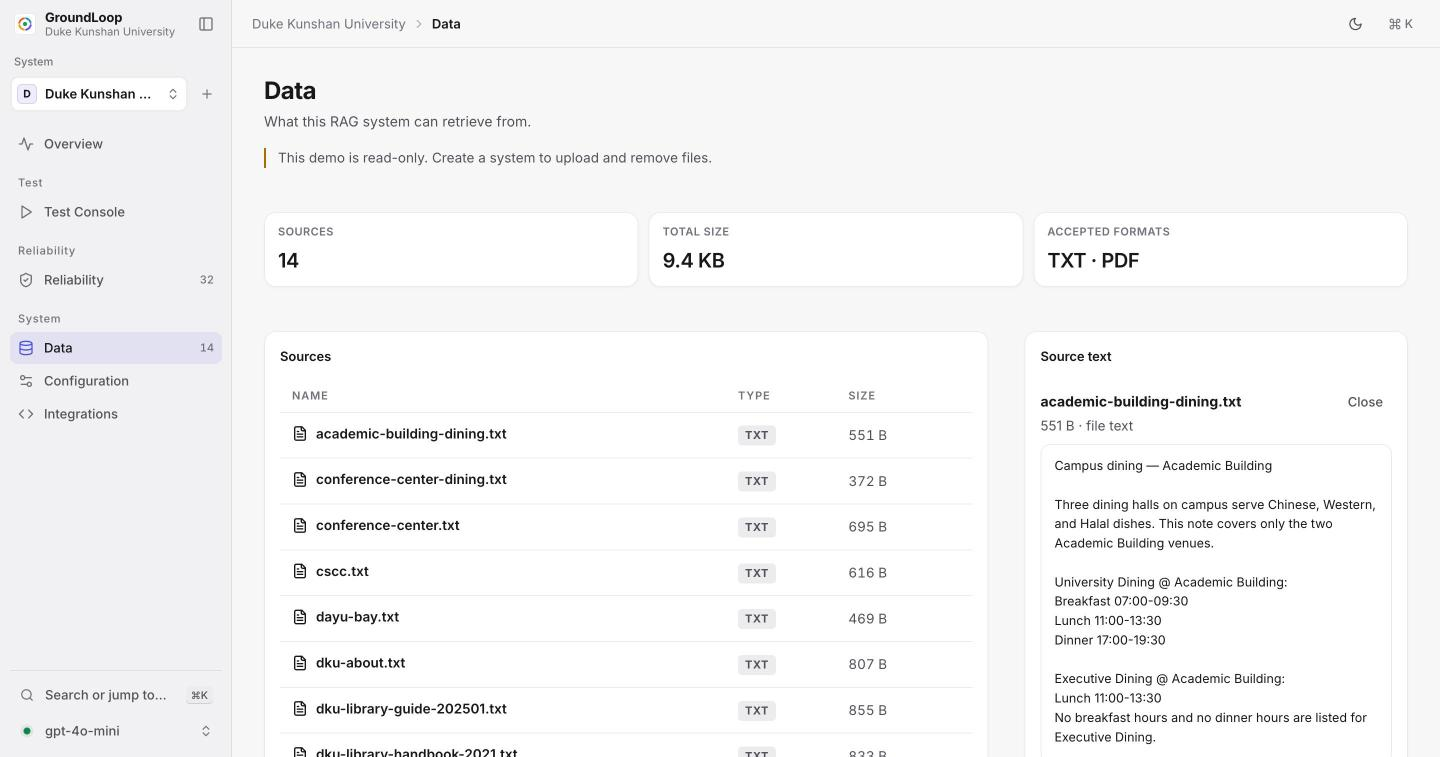
\includegraphics[width=0.8\textwidth]{figures/data.jpg}
\caption{The Data page, listing a system's sources with one open.}
\label{fig:data}
\end{figure}

\begin{figure}[H]
\centering
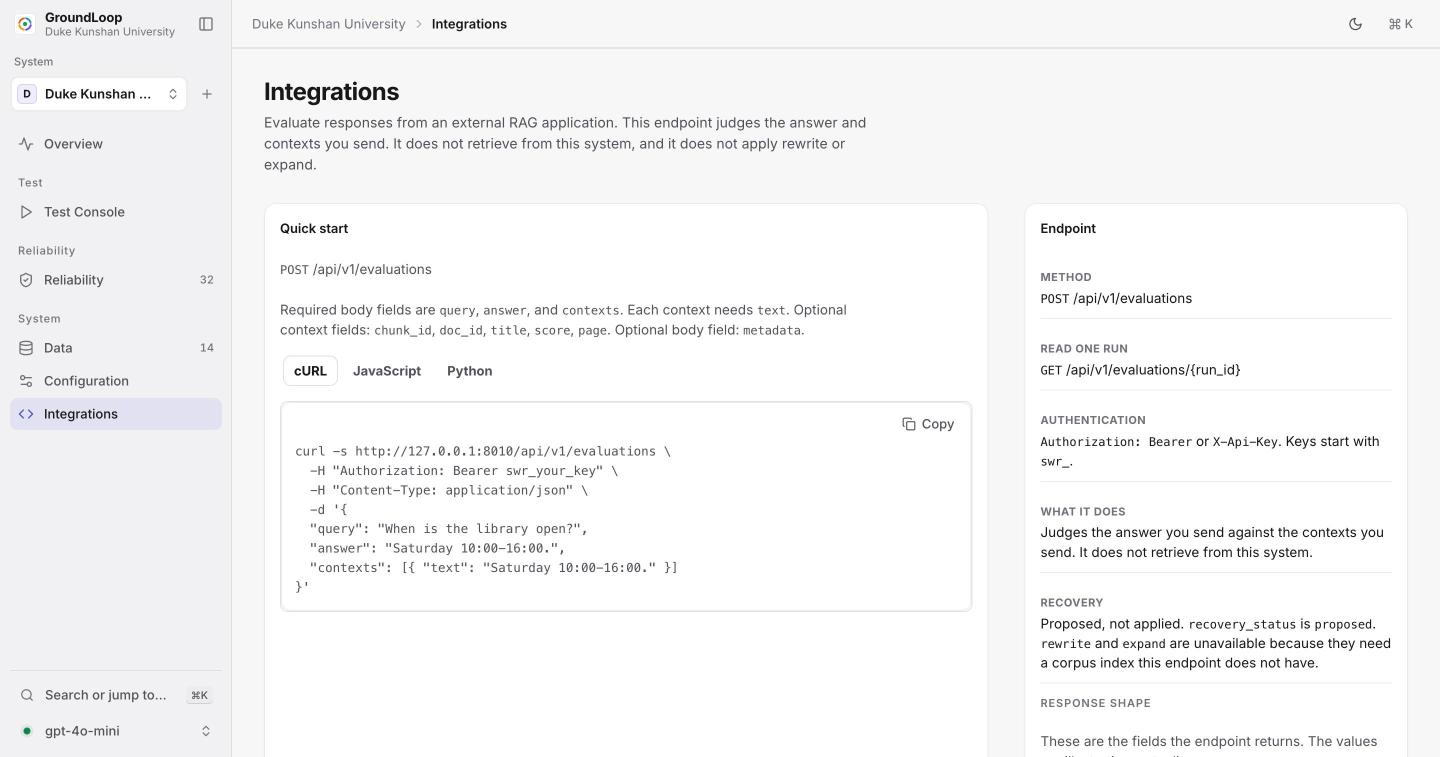
\includegraphics[width=0.8\textwidth]{figures/integrations.jpg}
\caption{The Integrations page for the external evaluation API.}
\label{fig:integrations}
\end{figure}

\end{document}
